% 导言区
\documentclass[12pt,a4paper,UTF8]{ctexart}
\usepackage{geometry}
\geometry{left=2.5cm,right=2.5cm,top=3.2cm,bottom=2.8cm}
\usepackage{amsmath,paralist,enumerate,booktabs,multirow,graphicx,float,subcaption,setspace,listings,lastpage,hyperref}
\usepackage{enumitem} % 添加 enumitem 包
\usepackage{fancyhdr}
\usepackage{float}

\pagestyle{fancy}
\rhead{油滴的布朗运动}
\lhead{实验报告}
\cfoot{Page \thepage/\pageref{LastPage}}
\rfoot{\today}
\renewcommand{\headrulewidth}{0.4pt}
\renewcommand{\theenumi}{\arabic{enumi}.} % 设置 enumerate 环境的编号格式为 1.
\setlist[enumerate,1]{label=\arabic*.} % 使用 enumitem 包设置编号格式

\setlength{\parindent}{2em}



\begin{document}

\section*{油滴的布朗运动实验报告}

\subsection*{实验名称}
油滴的布朗运动

\subsection*{实验目的}
\begin{enumerate}
    \item 验证布朗运动的基本特征： 
	\begin{equation}
    		\langle x(t)\rangle =0 ,
		\langle x^2(t)\rangle =2Dt
	\end{equation}
    \item 测量悬浮油滴颗粒的扩散系数 D
    \item 掌握利用CCD显微密立根油滴仪进行实验数据采集和分析的方法
\end{enumerate}

\subsection*{实验仪器}
密立根油滴实验装置、油滴喷雾器、温度计

油滴实验装置是油滴盒，油滴照明装置，调平系统，测量显微镜，供电电源以及电子停表，喷雾器等组成的，其实验装置如图1所示。
其中油滴盒，是由两块经过精磨的金属平板中间垫以胶木圆环构成的平行板电容器。在上板中心处有落油孔，使微小油滴可以进入电容器中间的电场空间，胶木圆环上有进光孔，观察孔。进入电场空间内的油滴由照明装置照明，油滴盒可通过调平螺旋调整水平，用水准仪检查。油滴盒防风罩前装有测量显微镜，并连接 CCD 。
\begin{figure}[h]
    \centering
    
\includegraphics[width=0.5\textwidth]{1}
    \caption{油滴实验装置图}
   \label{fig:example}
\end{figure}

其中，1-油雾室，2-油雾孔开关，3-防风罩，4-上电极板，5-胶木圆环，6-下电极板，7-底板，8-上盖板，9-喷雾口，10-油雾孔，11-上电极板压簧，12-上电极板电源插孔，13-油滴盒基座

\subsection*{实验原理}

\begin{enumerate}
    \item 布朗运动的含义

布朗运动是指悬浮在液体或气体中的微粒所做的永不停息的无规则运动。因由英国植物学家罗伯特·布朗所发现而得名。作布朗运动的微粒直径一般为 $10^{-5} \sim 10^{-3}$ 厘米，这些小的微粒处于液体或气体中时，由于分子的热运动，微粒受到来自各个方向分子的碰撞，当受到不平衡的冲撞时而运动，由于这种不平衡的冲撞，微粒的运动不断地改变方向而使微粒出现不规则的运动。布朗运动的剧烈程度随着流体的温度升高而增加。
    \item 布朗运动规律

将粒子的布朗运动分为多次极短时间内的运动，$R_N$ 是
经过N次运动后离开原点的位移矢量，则离原点的方均距离正比于步数N。即
\begin{equation}
		\langle R_N^2\rangle =NL^2
	\end{equation}

L是每次运动的长度。由于碰撞次数正比于时间，所以方均距离也正比于时间,即
\begin{equation}
		\langle R_N^2\rangle =ct
	\end{equation}

每继续运动一次，距离的平方平均增加L。因为
\begin{equation}
		R_N=R_{N-1}+L
	\end{equation}
则得到
\begin{equation}
		\langle R_N^2\rangle =R_{N-1}^2+2R_{N-1}L+L^2
	\end{equation}
对许多走法作平均后，有
\begin{equation}
		\langle R_N^2\rangle =\langle R_{N-1}^2\rangle +L^2
	\end{equation}
由于 $\langle R_{N-1}L\rangle=0$ ,利用归纳法，即可得到
\begin{equation}
		\langle R_N^2\rangle =NL^2
	\end{equation}

	\item 爱因斯坦对布朗运动的研究

爱因斯坦的成果大体上可分两方面。

一是，根据分子热运动原理推导：在t时间里，微粒在某一方向上位移的统计平均值，即方均根值, $\langle R^2 \rangle=2Dt$ ，D是微粒的扩散系数。这一公式是看来毫无规则的布朗运动服从分子热运动规律的必然结果。

二是，对于球形微粒，推导出扩散系数公式。式中的 $\eta$ 是介质粘度，r是微粒半径, $k_B$是玻尔兹曼常数，T是环境温度。按此公式，只要实际测得准确的扩散系数D或布朗运动均方位移就可得到原子和分子的绝对质量。爱因斯坦曾用前人测定的糖在水中的扩散系数，估算的 $N_A$ 值为 $3.3 \times 10^{23}$ ，一年后（1906），又修改为 $6.56 \times 10^{23}$ 。

扩散系数公式如下，
\begin{equation}
		D=\frac{k_B T}{6 \pi \eta r}
	\end{equation}

	\item 静态法验证布朗运动规律

通过静态法可以为验证上述两条布朗运动规律方程，并测量油滴的扩散系数 $\eta$和半径r。

实验研究对象是带电的油滴，基本思想是使油滴处于受力平衡状态。
当油滴受力平衡时，可视为在竖直方向上静止不动，因此我们可以追踪粒子在水平方向上的一维布朗运动,通过实验数据验证上式。
油滴通过喷雾器喷射进入两块相距为d的平行极板之间。油在喷射撕裂成油滴时，一般都是带电的。如果调节两极板之间的电压U,可使油滴悬浮在空中，如图2所示。设油滴的质量为m，所带的电量为q，两极板间的电压为U，则油滴在平行极板之间所受重力mg，静电力$qE=\frac{qU}{d}$。

\begin{figure}[h]
    \centering
    
\includegraphics[width=0.4\textwidth]{2}
    \caption{带电油滴受力图}
   \label{fig:example}
\end{figure}
因m很小，难直接测量。油滴可视为球状，设密度为$\rho$，油滴的质量m可表示为
\begin{equation}
		m=\rho \frac{4}{3}\pi r^3
	\end{equation}
而油滴的半径r可通过其在重力场中的终极速度求出。
平行极板不加电压时，油滴受重力作用而加速下降，由于空气阻力的作用,
下降一段距离达到某一速度 后，阻力$f_r$与重力mg平衡，如图3所示（空气浮力忽略不计），油滴将匀速下降。$v_g$称为终极速度。
\begin{figure}[h]
    \centering
    
\includegraphics[width=0.4\textwidth]{3}
    \caption{油滴受力平衡图(E=0)}
   \label{fig:example}
\end{figure}

根据斯托克斯定律，
\begin{equation}
		f_r=6 \pi r \eta v
	\end{equation}
其中$\eta$是空气的粘滞系数，r是油滴的半径。
重力mg与阻力$f_r$平衡时,
\begin{equation}
	f_r=mg
	\end{equation} 
由式(9)(10)(11)得到油滴的半径，
\begin{equation}
    r = \sqrt{\frac{9 \eta v_g}{2 \rho g}}
\end{equation}

当两极板间的电压 \( U \) 为零时，油滴匀速下降的距离为 \( l \)，时间为 \( t_g \)，则油滴的匀速下降速度 \( v_g \) 为：
\begin{equation}
    v_g = \frac{l}{t_g}
\end{equation}

% 公式 (6)
结合以上公式，油滴的半径 r 可表示为：
\begin{equation}
    r = \sqrt{\frac{9 \eta l}{2 \rho g t_g}}
\end{equation}

% 公式 (7)
斯托克斯定律是以连续介质为前提的，对于半径小到$10^{-6}$m的微小油滴，已不能将空气看作连续介质，空气的粘滞系数应作如下修正：
空气的粘滞系数修正公式：\begin{equation}
    \eta' =  \frac{\eta}{1 + \frac{b}{p r}}
\end{equation}
其中 $b$ 是修正常数，$p$ 为大气压强。

已知参数：

\begin{align*}
h &= 0.008237\, \text{V} \, \text{m}, \\
\rho &= 981 \, \text{kg/m}^3, \\
g &= 9.79 \, \text{m/s}^2, \\
\eta &= 1.83 \times 10^{-5} \, \text{kg/(m} \cdot \text{s)}, \\
p &= 1.013 \times 10^5 \, \text{Pa}, \\
d &= 5.00 \, \text{mm}, \\
l &= 1.6 \, \text{mm}.
\end{align*}

待测参数为平衡电压 $U$ 及下落时间 $t_g$。

\end{enumerate}

\subsection*{实验内容}
\begin{enumerate}
    \item 用温度计记录开始实验与结束实验时的温度。
    \item 仪器调整

	调节仪器面板上的三只平衡旋钮，将平行电极板调到水平。打开仪器和显示器开关，按
“确认”键，选“平衡法”，进入测量界面。

    \item 测量前的练习

(1)熟悉操作按键。按键1：计时开始/结束。按键2：0V/工作，电压在0V和工作状态之间切换。按键3：平衡/提升，工作电压可在平衡电压和提升电压之间切换，提升电压比平衡电压高约200V。

(2)练习控制油滴平衡。用喷雾器向油滴盒内喷油，仔细调节“电压调节”旋钮，使油滴置于分划板上某条横线附近，以便准确判断出这颗油滴是否平衡了。注意：不要连续喷多次，以防堵塞极板上的小孔。
    \item 正式测量

测量时，选取在显示屏中的清晰油滴，平衡电压为150-250V,匀速下落1.6mm的
时间为20s左右。此时，油滴电量q和不确定度均较小。

要求测3个不同的油滴。
将按键2置于工作，按键3置于平衡，将电压调至200V左右。向油雾口喷油，调节显微镜旋钮，寻找移动缓慢的油滴，细调“电压调节”，使油滴处于静止状态。记录此时的平衡电压U。将按键3切换为“提升”，使油滴上升至顶部网格线，然后将按键3切换为“平衡”使油滴静止。

然后按下按键2，使电压为“0V”,油滴匀速下降。当下降到0格线时，迅速按下计时按钮，开始计时，待油滴下落至1.6mm格线，停止计时。记下油滴匀速下降的时间 $t_g$ 。
测量完一次后，使油滴上升至顶部格线。

对同一颗油滴应测3次 $t_g$ ,测完后对 $t_g$ 取平均值。

	\item 计算油滴半径

根据公式(13)(14)(15)
计算出油滴的半径

	\item 拍摄视频

	调整CCD显微密立根油滴仪，确保能清晰观察到悬浮在流体中的微粒。

	用摄像设备记录微粒的运动，拍摄视频。

	\begin{enumerate}[label=\roman*.]
            \item 验证位移均值关系

用以上测量得到的不同半径的3个油滴，分别录制5组视频记录油滴布朗运动情况。每组视频120s，以1秒为间隔，记录油滴的位置数据。
（由于录制过程中帧数存在不稳定的情况，真实间隔为1.004秒；但仍可保证间隔时间一致）
            \item 验证位移平方均值关系

用以上测量得到的不同半径的3个油滴，分别录制0-5秒、0-10秒、0-15秒、0-20秒、0-25秒、0-30秒的视频记录油滴布朗运动情况。不同时间间隔各自测量10组。
总计录制180个视频。每组视频取开头与结尾，记录油滴的位置数据。

保证每个视频中油滴运动相互独立，不存在时间间隔的重叠。
        \end{enumerate}
	\item 视频分析

	用追踪软件（Tracker）导入视频，追踪微粒的运动轨迹。
	分别记录3个油滴的位移随时间变化数据，选取视频的时间间隔相互独立，分别用于验证两个布朗运动规律。
	
	\item 数据处理

计算每组数据不同时间间隔的位移均值$\langle x(t)\rangle$

计算每组数据不同时间间隔的位移平方均值$\langle x^2(t)\rangle$

用Origin软件线性拟合绘制每组数据位移平方均值$\langle x^2(t)\rangle$与时间t的关系图

计算每组数据的不确定度，并进行比较

计算并验证扩散系数D

如果每组数据的结果的理论值与实际值相差过大，分析其原因

\end{enumerate}

\subsection*{数据记录}
\begin{enumerate}
\item 温度测量

实验前环境温度为 $23.2 ^\circ C$ ，实验后环境温度为 $23.1 ^\circ C$

取平均温度 $T=23.2 ^\circ C$

\item 油滴下落时间

\begin{table}[htbp]
  \centering
  \begin{tabular}{cccccc}
    \toprule
    油滴编号 & $U$ (V) & $t_{g1}$ (s) & $t_{g2}$ (s) & $t_{g3}$ (s) & 平均 $t_{g}$ (s) \\
    \midrule
    1 &79 &31.00 &31.26 &31.60 &31.29 \\
    2 &176 &28.60 &28.51 &28.55 &28.55 \\
    3 &129 &27.65 &27.33 &27.34 &27.44 \\
    \bottomrule
  \end{tabular}
  \caption{不同油滴的下落时间}
  \label{tab:data}
\end{table}

\item 位移均值测量数据

\begin{figure}[H]
	\centering
	\begin{subfigure}{0.2\textwidth}
		\centering
		
\includegraphics[width=\textwidth]{11}
		\caption{油滴1-1}
	\end{subfigure}
	\qquad
	\begin{subfigure}{0.2\textwidth}
		\centering
		
\includegraphics[width=\textwidth]{12}
		\caption{油滴1-2}
	\end{subfigure}
	\begin{subfigure}{0.185\textwidth}
		\centering
		
\includegraphics[width=\textwidth]{13}
		\caption{油滴1-3}
	\end{subfigure}
	\caption{油滴1位置与时间数据表}
\end{figure}

\begin{figure}[H]
	\centering
	\begin{subfigure}{0.2\textwidth}
		\centering
		
\includegraphics[width=\textwidth]{21}
		\caption{油滴2-1}
	\end{subfigure}
	\qquad
	\begin{subfigure}{0.2\textwidth}
		\centering
		
\includegraphics[width=\textwidth]{22}
		\caption{油滴2-2}
	\end{subfigure}
	\begin{subfigure}{0.185\textwidth}
		\centering
		
\includegraphics[width=\textwidth]{23}
		\caption{油滴2-3}
	\end{subfigure}
	\caption{油滴2位置与时间数据表}
\end{figure}

\begin{figure}[htbp]
	\centering
	\begin{subfigure}{0.2\textwidth}
		\centering
		
\includegraphics[width=\textwidth]{31}
		\caption{油滴3-1}
	\end{subfigure}
	\qquad
	\begin{subfigure}{0.2\textwidth}
		\centering
		
\includegraphics[width=\textwidth]{32}
		\caption{油滴3-2}
	\end{subfigure}
	\begin{subfigure}{0.185\textwidth}
		\centering
		
\includegraphics[width=\textwidth]{33}
		\caption{油滴3-3}
	\end{subfigure}
	\caption{油滴3位置与时间数据表}
\end{figure}

\item 位移平方均值测量数据

\begin{figure}[h]
    \centering
    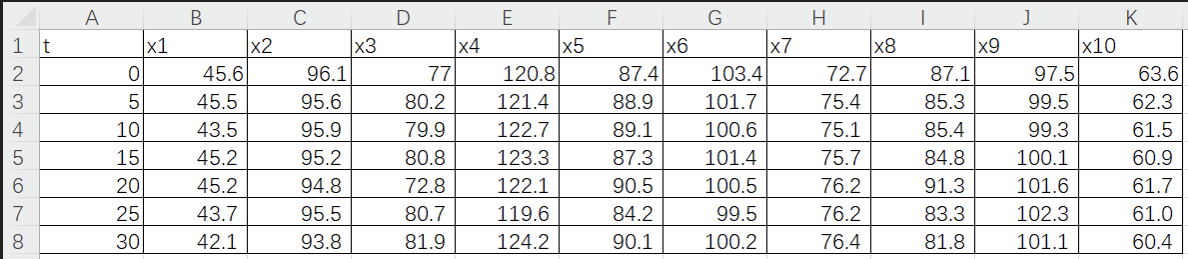
\includegraphics[width=0.5\textwidth]{010}
    \caption{油滴1位置数据}
   \label{fig:example}
\end{figure}

\begin{figure}[h]
    \centering
    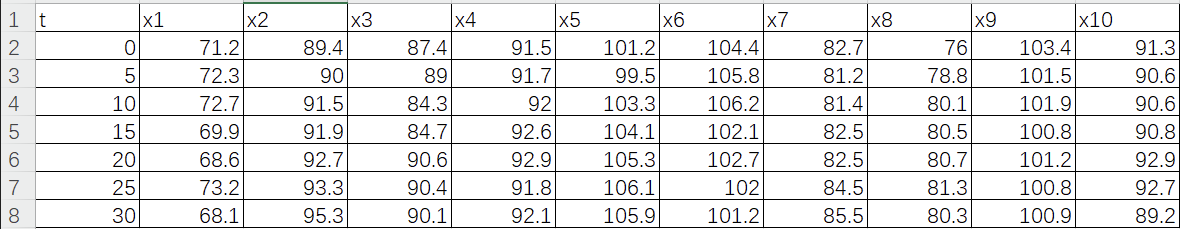
\includegraphics[width=0.5\textwidth]{020}
    \caption{油滴2位置数据}
   \label{fig:example}
\end{figure}

\begin{figure}[H]
    \centering
    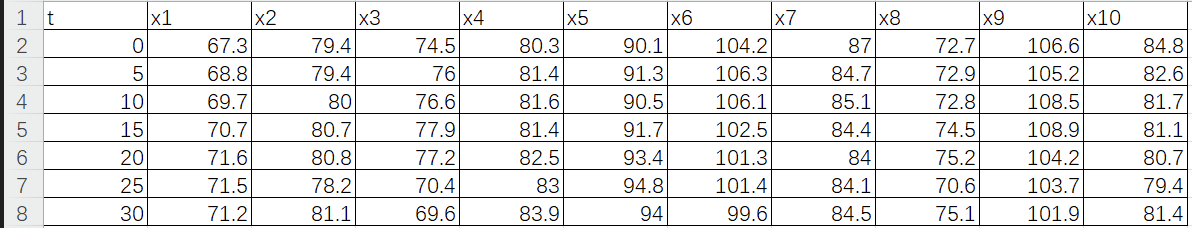
\includegraphics[width=0.5\textwidth]{030}
    \caption{油滴3位置数据}
   \label{fig:example}
\end{figure}


\end{enumerate}

\subsection*{数据处理}
\begin{enumerate}
\item 位移均值

\begin{figure}[htbp]
	\centering
	\begin{subfigure}{0.2\textwidth}
		\centering
		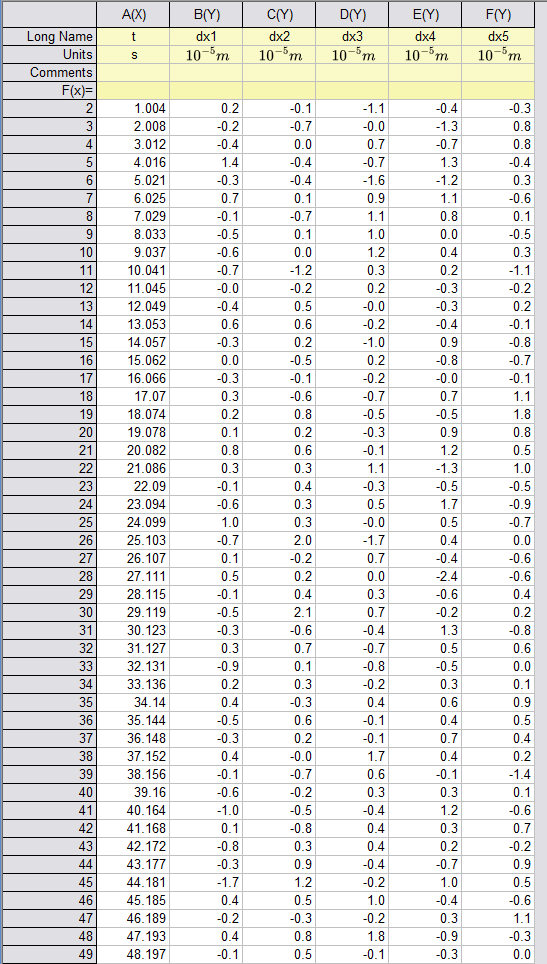
\includegraphics[width=\textwidth]{011}
		\caption{油滴1-1}
	\end{subfigure}
	\qquad
	\begin{subfigure}{0.2\textwidth}
		\centering
		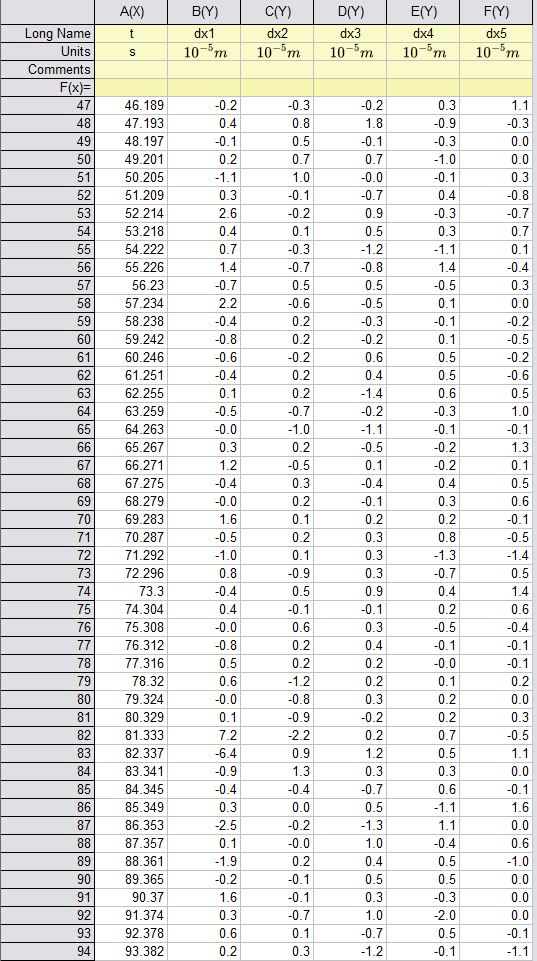
\includegraphics[width=\textwidth]{012}
		\caption{油滴1-2}
	\end{subfigure}
	\begin{subfigure}{0.185\textwidth}
		\centering
		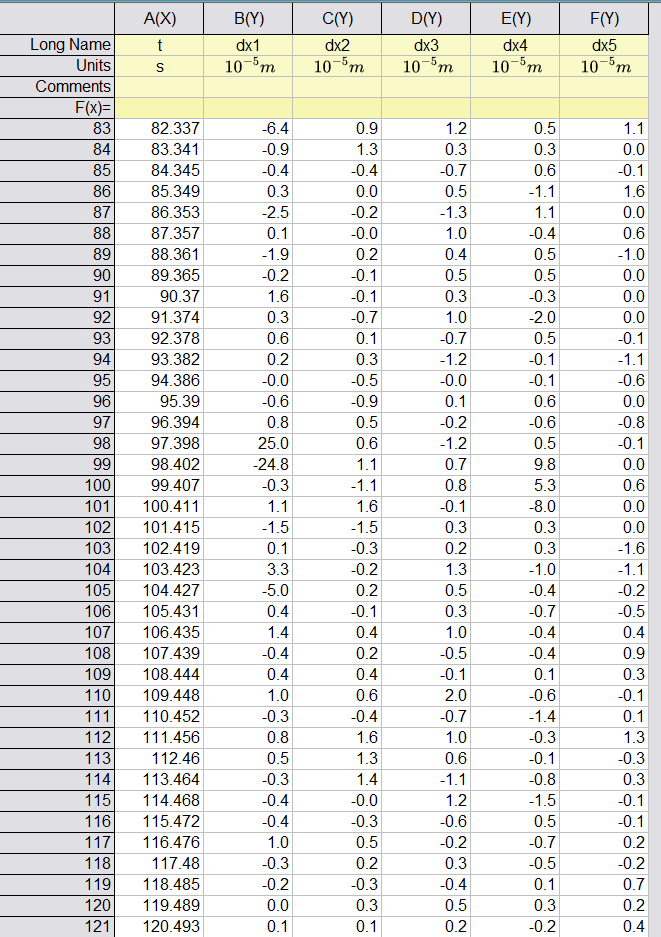
\includegraphics[width=\textwidth]{013}
		\caption{油滴1-3}
	\end{subfigure}
	\caption{油滴1位移数据表}
\end{figure}

\begin{figure}[htbp]
	\centering
	\begin{subfigure}{0.2\textwidth}
		\centering
		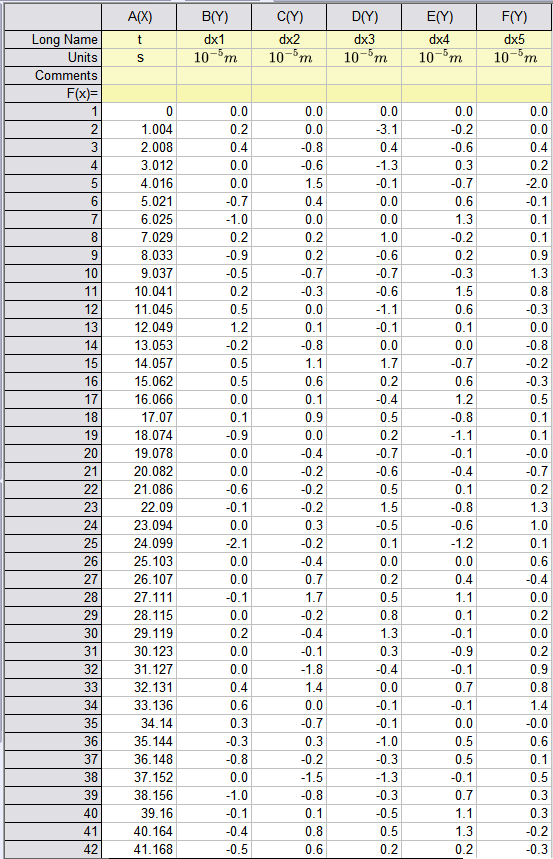
\includegraphics[width=\textwidth]{021}
		\caption{油滴2-1}
	\end{subfigure}
	\qquad
	\begin{subfigure}{0.2\textwidth}
		\centering
		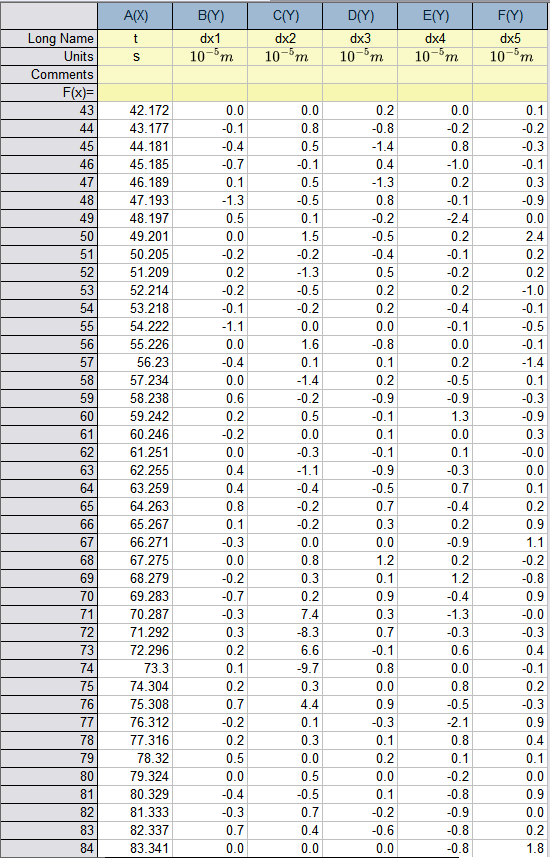
\includegraphics[width=\textwidth]{022}
		\caption{油滴2-2}
	\end{subfigure}
	\begin{subfigure}{0.185\textwidth}
		\centering
		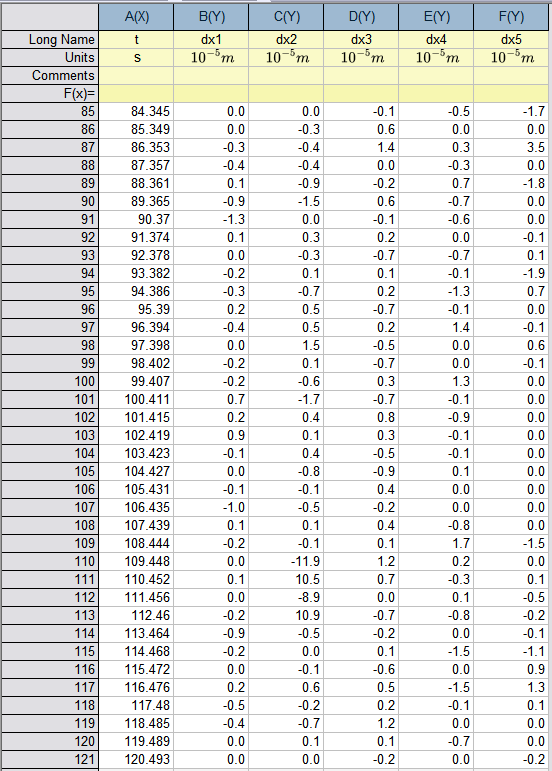
\includegraphics[width=\textwidth]{023}
		\caption{油滴2-3}
	\end{subfigure}
	\caption{油滴2位移数据表}
\end{figure}



\begin{figure}[H]
	\centering
	\begin{subfigure}{0.2\textwidth}
		\centering
		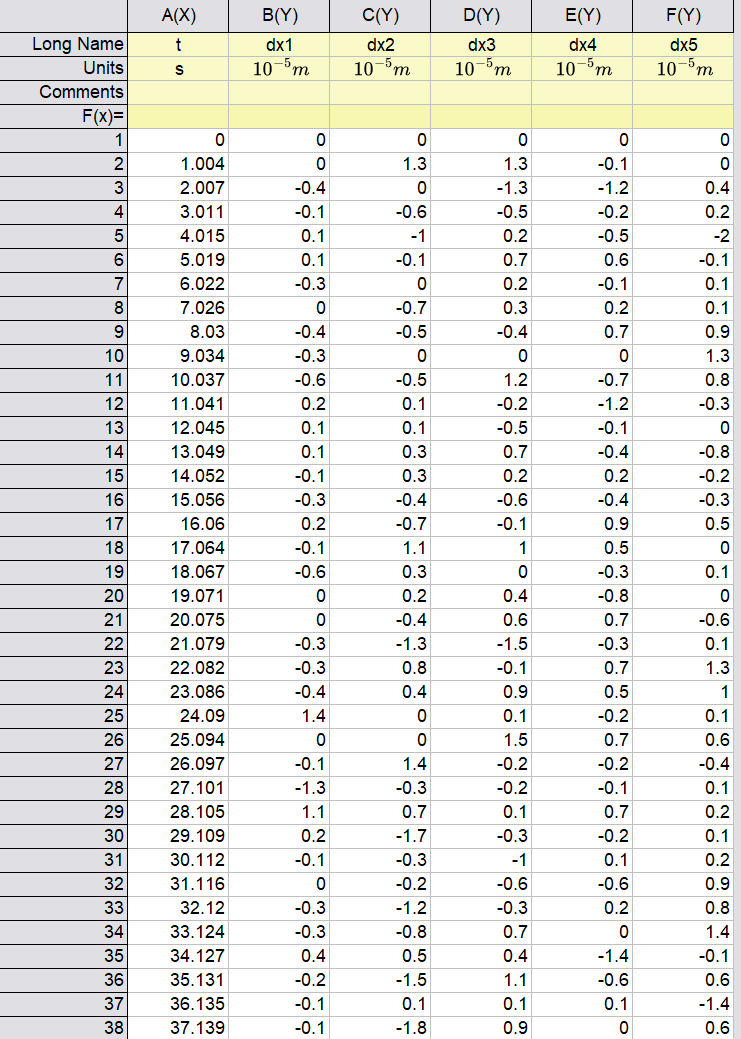
\includegraphics[width=\textwidth]{031}
		\caption{油滴3-1}
	\end{subfigure}
	\qquad
	\begin{subfigure}{0.2\textwidth}
		\centering
		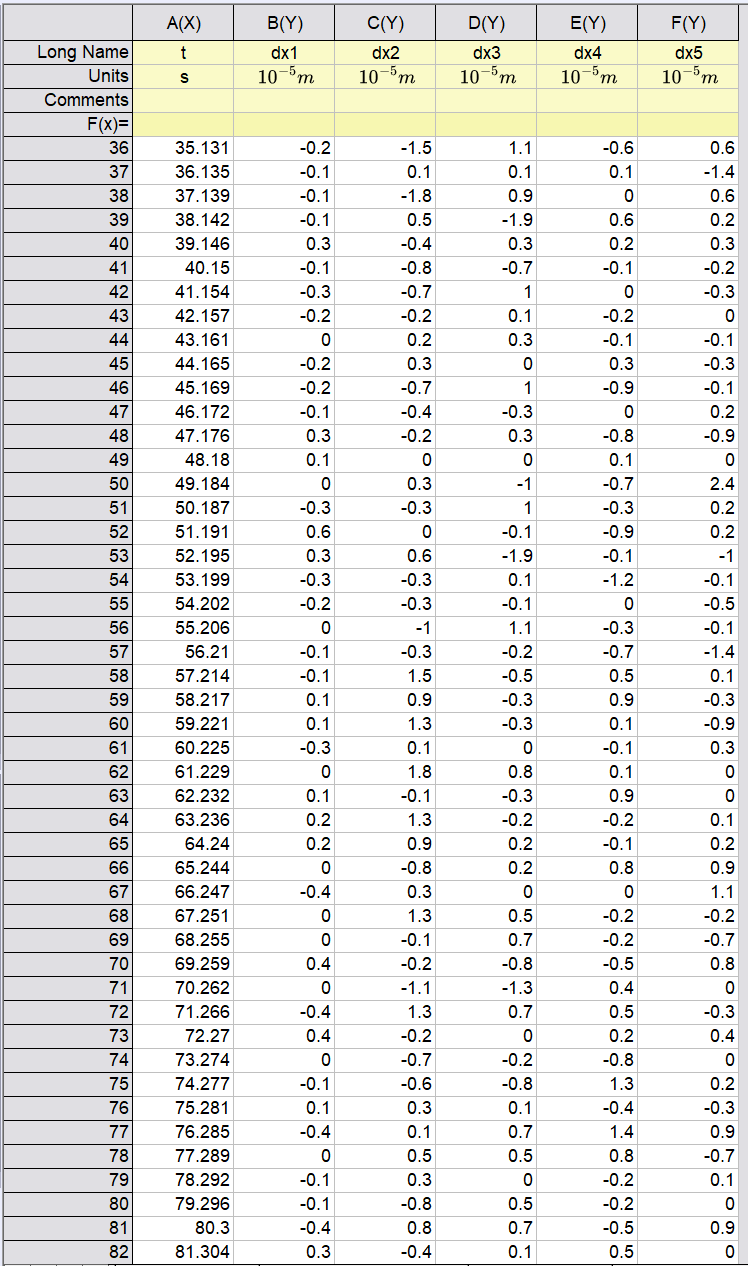
\includegraphics[width=\textwidth]{032}
		\caption{油滴3-2}
	\end{subfigure}
	\begin{subfigure}{0.185\textwidth}
		\centering
		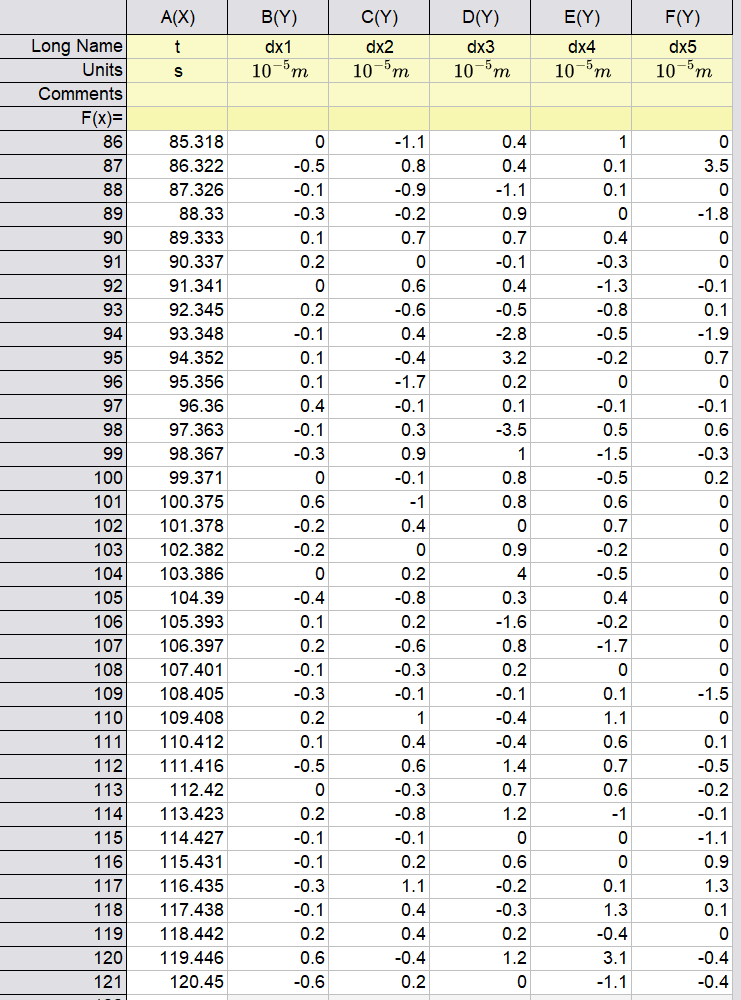
\includegraphics[width=\textwidth]{033}
		\caption{油滴3-3}
	\end{subfigure}
	\caption{油滴3位移数据表}
\end{figure}

\begin{figure}[h]
    \centering
    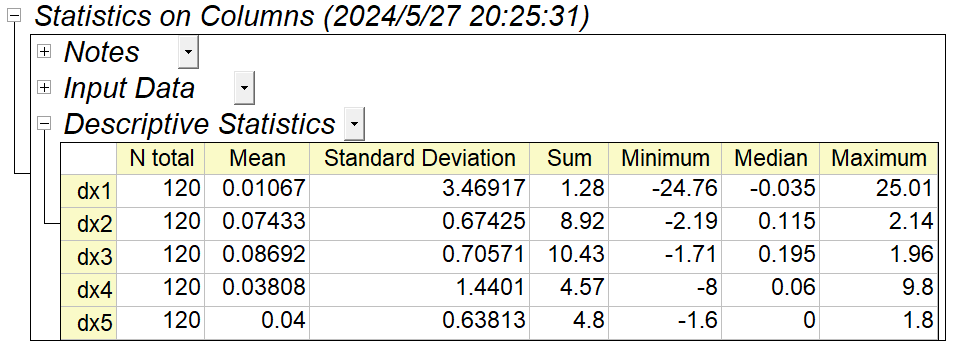
\includegraphics[width=0.5\textwidth]{014}
    \caption{油滴1位移均值}
   \label{fig:example}
\end{figure}

\begin{figure}[h]
    \centering
    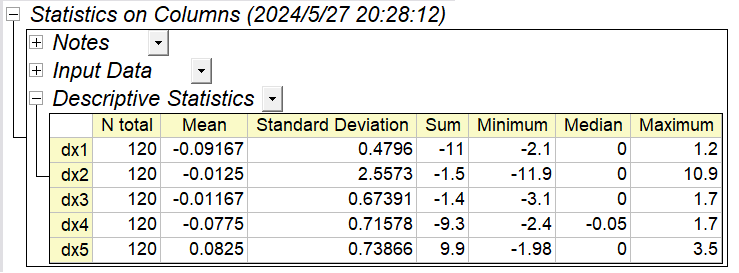
\includegraphics[width=0.5\textwidth]{024}
    \caption{油滴2位移均值}
   \label{fig:example}
\end{figure}

\begin{figure}[H]
    \centering
    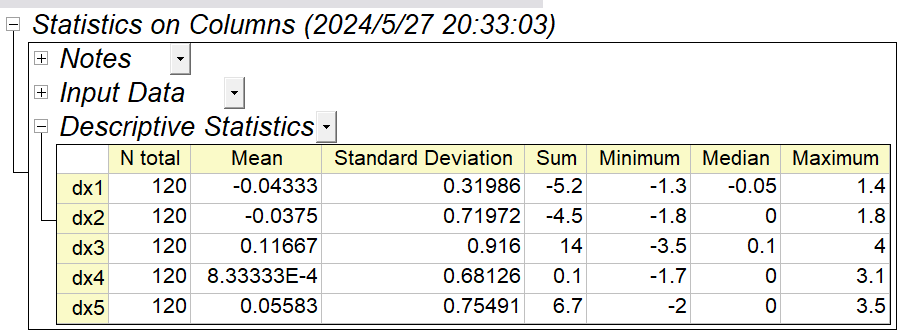
\includegraphics[width=0.5\textwidth]{034}
    \caption{油滴3位移均值}
   \label{fig:example}
\end{figure}
由位移均值的计算，初步验证了位移均值接近0，符合布朗运动规律。

\item 位移的不确定度\par
本实验中，分别测量了3个油滴的5组轨迹位移量，每组120个实验数据，共计1800个数据。
利用不确定度来分析测量位移的平均值，从实验控制误差的角度，通常需要考虑测量的最大不确定度。
实验在相同的的条件下对油滴的每个时刻的位移进行了多次测量，可以进行不确定度的计算。
\par
$u_{A}$为测量列的A类标准不确定度，即测量列的平均值的标准差，由概率论公式可得，算术平均值 $\overline{x}$的标准差$u_{A}$为
\par
\begin{equation}
u_{A}=\frac{\sigma}{\sqrt{n}}
\end{equation}
在A类不确定度$u_{A}$公式中，标准差$\sigma$为
\par
\begin{equation}
\sigma=\sqrt{\frac{\sum\limits_{i=1}^{k}(\overline{x}-x_{i})}{n-1}}
\end{equation}

$u_{B}$为做测量中不符合统计规律的不确定度，通常来自仪器的最大允差和估计读数的最大允差。

实验仪器中，秒表精度为0.01s，追踪软件（Tracker）长度测量精度为$1 \times 10^{-6}m$。

在本实验中，B类不确定度远小于A类不确定度，因此在不确定度的合成中，可以忽略B类不确定度。
\par
取置信概率P=0.95，查t分布表，取$t_{0.95}$=2

位移的展伸不确定度为 $u_{x,0.95}=t_{0.95}u_{A}$

根据置信概率P=0.95，测量结果的最终表达式为
\begin{equation}
\langle x\rangle=\overline{x}+u_{x,0.95}
\end{equation}

对第一颗油滴的数据进行数据分析，n=120\par
\begin{table}[htbp]
  \centering
  \begin{tabular}{cccccc}
    \toprule
    实验组数 &$\overline{x}$ &$\sigma$  & $u_{A}$&$u_{x,0.95} $\\
    \midrule
    1 &-0.09167&0.47796 &0.04378 &0.08756 \\
    2 &-0.0125&2.55730 &0.23345  &0.4669\\
    3 &-0.01167&0.67391 &0.06152  &0.12304\\
    4 &-0.0775&0.71578 &0.06534  &0.13068\\
    5 &0.0825&0.73866 &0.06743  &0.13486\\
    \bottomrule
  \end{tabular}
  \caption{油滴1的不确定度}
  \label{tab:data}
\end{table}
除了实验组1外，其余测量结果的最终表达式范围中均包括了$\langle x \rangle$=0,可以看出剩余四组的数据较为合理，符合布朗运动规律。


对第二颗油滴的数据进行数据分析，n=120
\par
\begin{table}[htbp]
  \centering
  \begin{tabular}{cccccc}
    \toprule
    实验组数 &$\overline{x}$ &$\sigma$  & $u_{A}$&$u_{x,0.95} $\\
    \midrule
    1 &0.01448&3.52880 &0.32764&0.65528  \\
    2 &0.07431&0.68456 &0.06356&0.12712 \\
    3 &0.08474&0.71504 &0.06639&0.13278  \\
    4 &0.04198&1.46369 &0.13590&0.27180  \\
    5 &0.0319&0.64473 &0.05986&0.11972  \\
    \bottomrule
  \end{tabular}
  \caption{油滴2的不确定度}
  \label{tab:data}
\end{table}
五组实验测量结果的最终表达式范围中均包括了$\langle x \rangle$=0,可以看出实验所得数据较为合理，符合布朗运动规律。
\par
对第三颗油滴的数据进行数据分析，n=120
\par
\begin{table}[htbp]
  \centering
  \begin{tabular}{cccccc}
    \toprule
   实验组数 &$\overline{x}$ &$\sigma$  & $u_{A}$&$u_{x,0.95} $\\
    \midrule
    1 &-0.04333&0.31986 &0.02920 & 0.0584\\
    2 &-0.0375&0.71972 &0.06570 &0.1314\\
    3 &0.11667&0.91600 &0.08362 & 0.16724\\
    4 &8.33333E-4&0.68126 &0.06219 &0.12438\\
    5 &0.05583&0.75491 &0.06891 &0.13783 \\
    \bottomrule
  \end{tabular}
  \caption{油滴3的不确定度}
  \label{tab:data}
\end{table}
五组实验测量结果的最终表达式范围中均包括了$\langle x \rangle$=0,可以看出实验所得数据较为合理，符合布朗运动规律。

由以上计算，可以得出油滴的运动情况符合布朗运动规律，在误差允许范围之内 $<x>=0$ .


\item 位移平方均值

\begin{figure}[H]
    \centering
    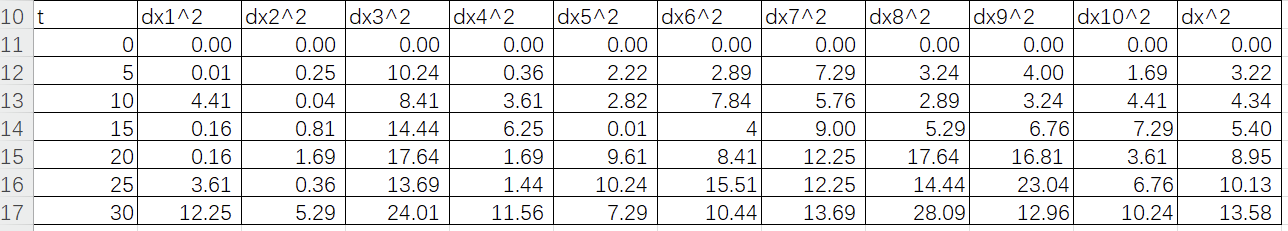
\includegraphics[width=0.5\textwidth]{019}
    \caption{油滴1位移平方}
   \label{fig:example}
\end{figure}

\begin{figure}[h]
    \centering
    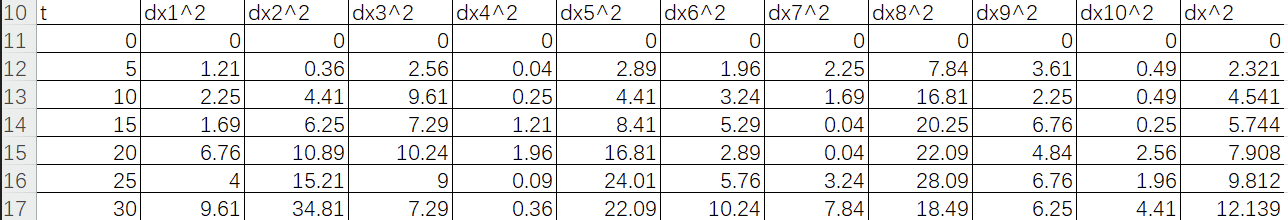
\includegraphics[width=0.5\textwidth]{029}
    \caption{油滴2位移平方}
   \label{fig:example}
\end{figure}

\begin{figure}[H]
    \centering
    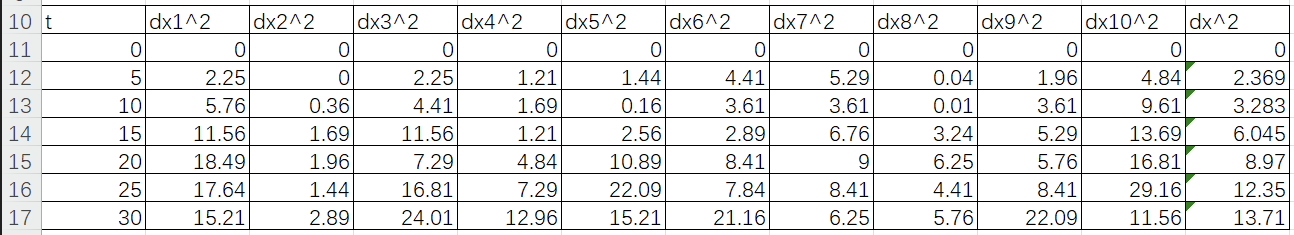
\includegraphics[width=0.5\textwidth]{039}
    \caption{油滴3位移平方}
   \label{fig:example}
\end{figure}

\item 位移平方均值与时间的线性拟合

\begin{figure}[H]
    \centering
    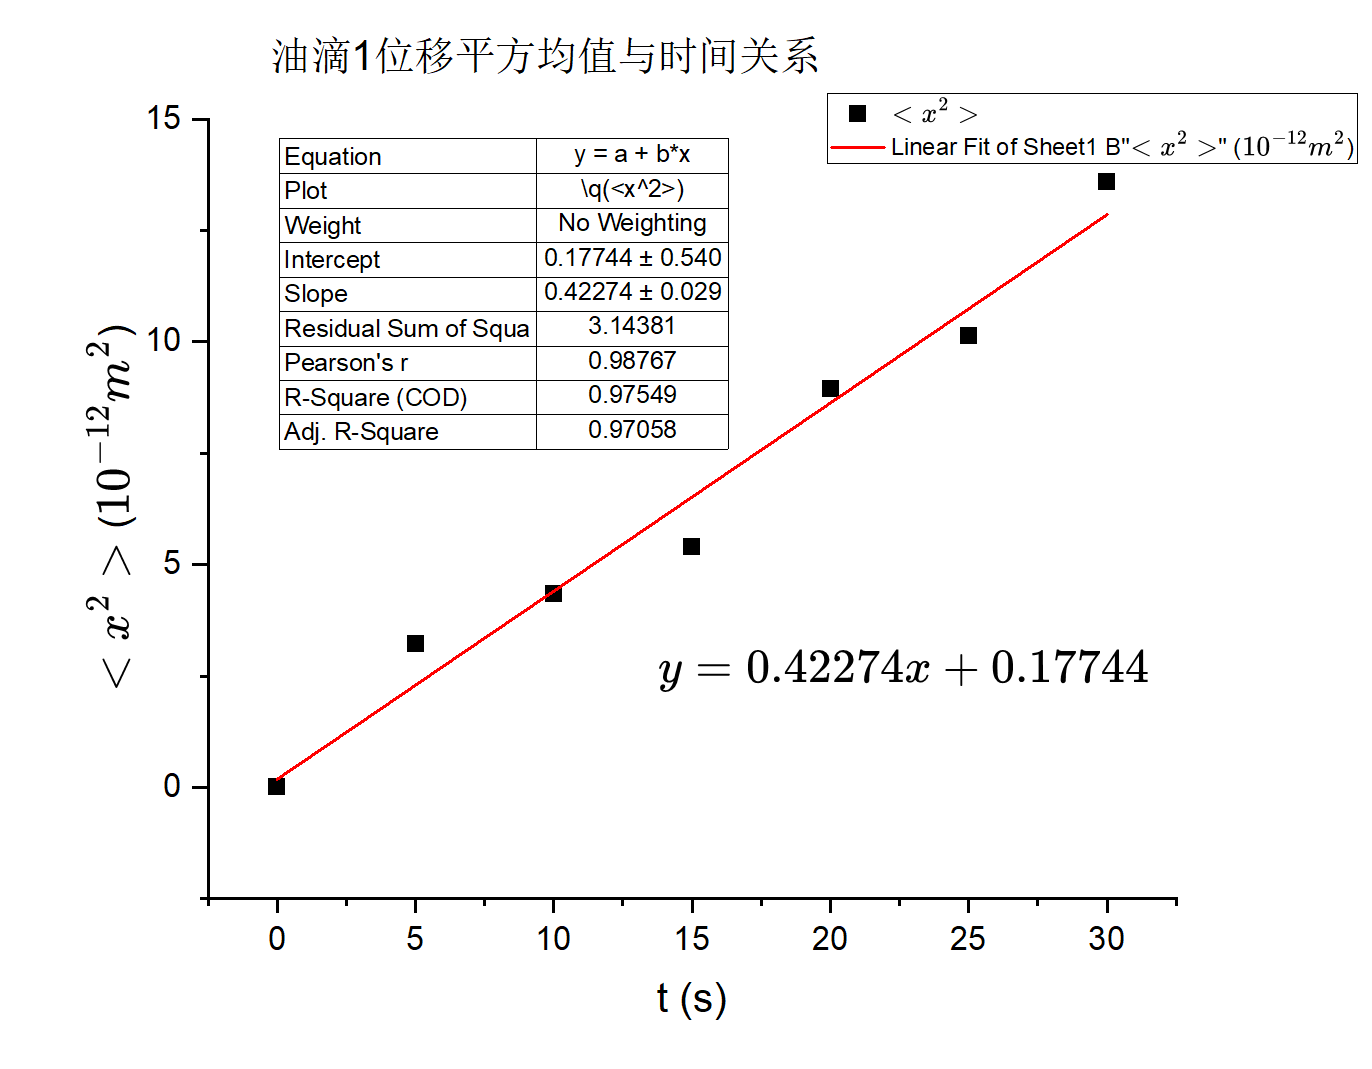
\includegraphics[width=0.5\textwidth]{f1}
    \caption{油滴1位移平方均值与时间的线性拟合}
   \label{fig:example}
\end{figure}

\begin{figure}[H]
    \centering
    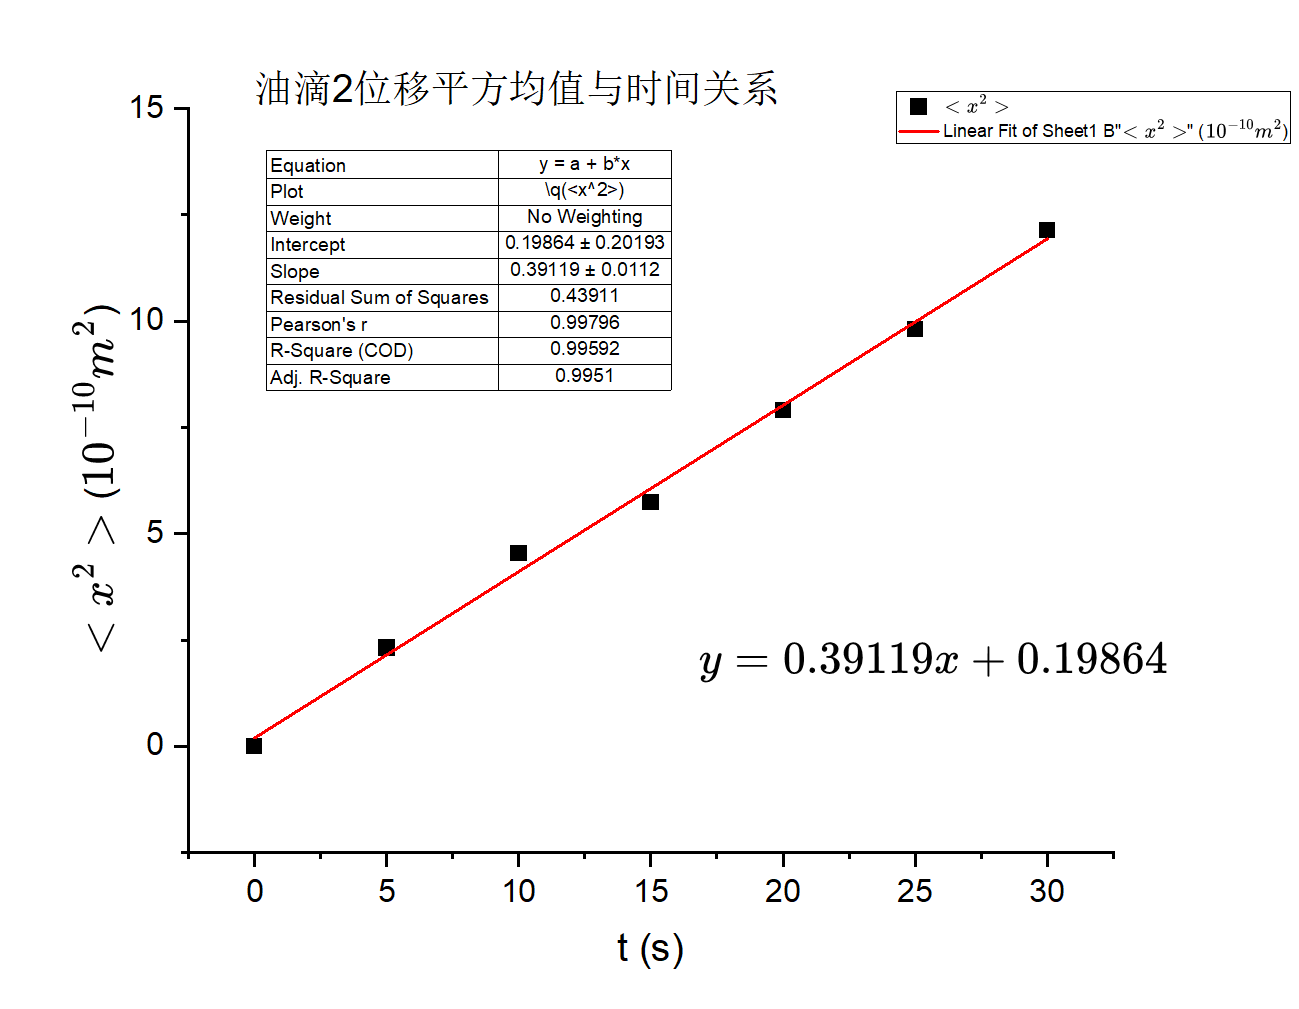
\includegraphics[width=0.5\textwidth]{f2}
    \caption{油滴2位移平方均值与时间的线性拟合}
   \label{fig:example}
\end{figure}

\begin{figure}[H]
    \centering
    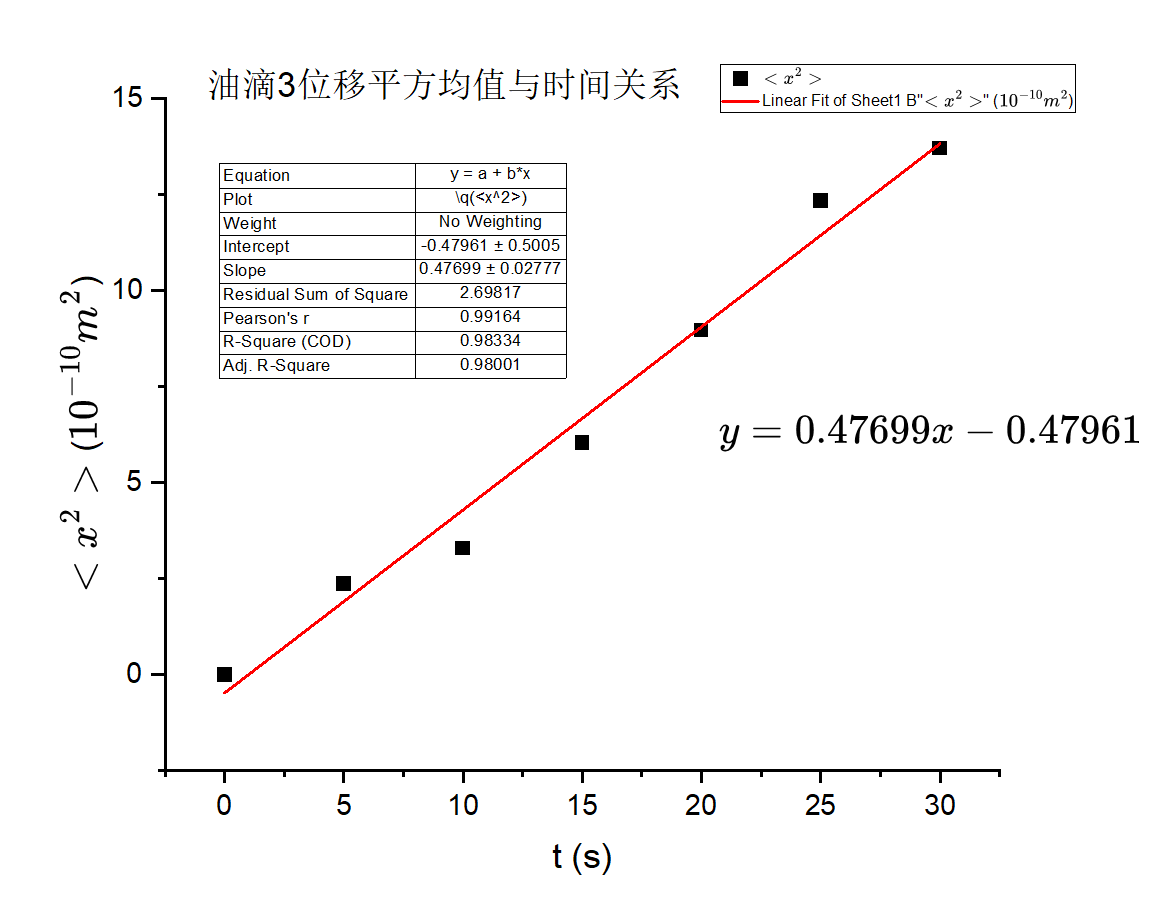
\includegraphics[width=0.5\textwidth]{f3}
    \caption{油滴3位移平方均值与时间的线性拟合}
   \label{fig:example}
\end{figure}

由拟合图像可知，在误差范围内，位移均值平方与时间成正比例关系，截距近似为0，符合布朗运动规律。

\item 计算并验证扩散系数
\begin{enumerate}[label=\roman*.]
            \item 由公式(14)(15)，联立方程，可计算得到油滴半径

            \item 再由扩散系数公式(8)，可计算得出不同半径油滴对应的扩散系数D的理论值

\begin{table}[htbp]
  \centering
  \begin{tabular}{cccccc}
    \toprule
    油滴编号 & 平均 $t_{g}$ (s) &油滴半径 r$(nm)$ &扩散系数 D $(10^{-12}m^2)$\\
    \midrule
    1 &31.29 &622.8 &21.53  \\
    2 &28.55 &653.8 &20.40 \\
    3 &27.44 &667.6 &19.93  \\
    \bottomrule
  \end{tabular}
  \caption{不同油滴的半径及扩散系数}
  \label{tab:data}
\end{table}

	\item 通过线性拟合图像计算扩散系数实验值

由公式 $\langle R^2 \rangle=2Dt$ ，计算扩散系数实验值

\begin{table}[htbp]
  \centering
  \begin{tabular}{cccccc}
    \toprule
    油滴编号 &图像斜率k $(10^{-12}m^2)$ &扩散系数 D $(10^{-12}m^2)$\\
    \midrule
    1 &42.27 &21.14  \\
    2 &39.12 &19.56  \\
    3 &47.70 &23.85  \\
    \bottomrule
  \end{tabular}
  \caption{不同油滴的图像斜率及扩散系数实验值}
  \label{tab:data}
\end{table}

\item 将扩散系数D的理论值和实验值进行比较

用 $\frac{|D_{\text{实}} - D_{\text{理}}|}{D_{\text{理}}}\times 100\%$ ,估算测量到的扩散系数D是否在误差范围之内

\begin{table}[H]
  \centering
  \begin{tabular}{cccccc}
    \toprule
    油滴编号 &测量扩散系数 D $(10^{-12}m^2)$ &理论扩散系数 D $(10^{-12}m^2)$ & $\frac{|D_{\text{实}} - D_{\text{理}}|}{D_{\text{理}}}\times 100\%$\\
    \midrule
    1 &21.14 &21.53 &1.811\% \\
    2 &19.56 &20.40 &4.118\% \\
    3 &23.85 &19.93 &19.67\% \\
    \bottomrule
  \end{tabular}
  \caption{扩散系数理论值和实验值比较}
  \label{tab:data}
\end{table}
由上表可知，油滴1、2测量扩散系数与理论扩散系数相差较小，在误差允许范围内；油滴3测量扩散系数与理论扩散系数相差较大，存在一定误差。

\end{enumerate}

\end{enumerate}

\subsection*{误差分析}
\begin{enumerate}
	\item 仪器误差

CCD显微密立根油滴仪：分辨率限制导致位置测量不精确。
显微镜的分辨率决定了微粒位置的测量精度，分辨率不足可能导致位移数据的偏差。

改进方法是使用更高分辨率的显微镜。
	\item 数据分析误差

追踪软件的识别精度有限。追踪软件可能无法准确追踪微粒的运动轨迹，特别是在微粒速度较快或图像质量较差的情况下。

改进方法是使用高精度的追踪算法，并手动校正自动追踪结果。
	\item 温度环境误差

实验中温度波动可能导致扩散系数测量不准确。

改进方法是在恒温环境下进行实验，使用恒温设备保持实验温度稳定。
	\item 微粒半径测量

微粒半径的测量误差直接影响扩散系数的计算。微粒半径测量不准确会导致扩散系数计算结果偏差。

改进方法是对微粒半径进行多次测量，取平均值，减小测量误差。

	\item 系统误差

理论模型假设简化了实际情况，例如忽略了流体中的其他力（如重力、浮力等）对微粒运动的影响。这些简化假设可能导致实验结果与实际情况存在系统性偏差。

改进方法是考虑更多实际因素，完善理论模型。
	
	\item 数据处理误差

数据处理过程中存在拟合误差。在拟合时，数据点的分布和拟合曲线的选择会影响拟合结果。如果数据点不够均匀或者存在异常值，拟合结果可能不准确。

改进方法是排除异常值，确保数据点均匀分布，并选择合适的拟合方法。

	\item 人为误差

在实验操作过程中，人为操作误差会影响实验结果，例如显微镜对焦不准、相机拍摄朝向与刻度线不完全垂直、录像时间间隔不一致等。

改进方法是严格按照实验步骤进行操作，减少人为误差。
\end{enumerate}
\subsection*{实验结论}
本实验通过利用密立根油滴实验装置，测量了油滴随时间的位移数据，对油滴在空气中的布朗运动规律进行研究。

实验验证了布朗运动的基本特征，在误差范围内
$\langle x(t)\rangle =0 ,\langle x^2(t)\rangle =2Dt$ ,
测量结果均满足上式。

实验测得三种不同半径油滴的扩散系数,与理论值较为接近，证明了实验方法的可行性；与理论值偏差较大的数据进行了误差分析。
\subsection*{拓展}
\begin{enumerate}
\item 通过扩散系数D计算玻尔兹曼常数$k_B$

由公式(8)变形得，
\begin{equation}
		k_B=\frac{6 \pi \eta r D}{T}
	\end{equation}
并使用公式(15)修正后的流体粘度 $\eta'$
由三组扩散系数计算得到玻尔兹曼常数$k_B$

\begin{table}[htbp]
  \centering
  \begin{tabular}{cccccc}
    \toprule
    油滴编号 &油滴半径 r$(nm)$ &测量扩散系数 D $(10^{-12}m^2)$ &玻尔兹曼常数 $k_B$ $(J/K)$\\
    \midrule
    1 &622.8 &21.14 & $1.356 \times 10^{-23}$ \\
    2 &653.8 &19.56 & $1.324 \times 10^{-23}$\\
    3 &667.6 &23.85 & $1.652 \times 10^{-23}$ \\
    \bottomrule
  \end{tabular}
  \caption{不同油滴测得的扩散系数及玻尔兹曼常数}
  \label{tab:data}
\end{table}

$\overline{k_B}=\frac{k_{B1}+k_{B2}+k_{B3}}{3}=1.444 \times 10^{-23}(J/K)$

观察表中数据，与标准值 $1.3806 \times 10^{-23}$相比，发现误差主要源于第三组数据。

\item 通过玻尔兹曼常数$k_B$得到阿伏伽德罗常数$N_A$

理想气体常数 $R=8.314J/(K \cdot mol)$

由 $N_{\text{A}} = \frac{R}{k}$ ,

\begin{table}[htbp]
  \centering
  \begin{tabular}{cccccc}
    \toprule
    油滴编号 &玻尔兹曼常数 $k_B$ $(J/K)$ & 阿伏伽德罗常数$N_A(mol^{-1})$\\
    \midrule
    1 & $1.356 \times 10^{-23}$ & $6.131 \times 10^{23}$ \\
    2 & $1.324 \times 10^{-23}$ & $6.279 \times 10^{23}$\\
    3 & $1.652 \times 10^{-23}$ & $5.033 \times 10^{23}$\\
    \bottomrule
  \end{tabular}
  \caption{不同油滴测得的玻尔兹曼常数及阿伏伽德罗常数}
  \label{tab:data}
\end{table}

$\overline{N_A}=\frac{N_{A1}+N_{A2}+N_{A3}}{3}=5.758 \times 10^{23}(mol^{-1})$

观察表中数据，与标准值 $6.0221 \times 10^{23}$相比，发现误差主要源于第三组数据。

\item 探究数据误差主要来源

测量实验主要由平衡法测量油滴半径、油滴布朗运动位移与时间两部分组成，通过对两个实验分别计算已经确定的标准量，分析得出主要误差来源。
油滴布朗运动位移与时间部分，已进行了实验扩散系数与测量扩散系数的比较。
平衡法测量油滴半径，可以通过计算元电荷的带电量，与元电荷标准量进行比较。

由公式(9)(14)(15),以及受力平衡方程 $\frac{qU}{d}=mg$,可以得到
\begin{equation}
q=\frac{18\pi}{\sqrt{2\rho g}}\left(\frac{\eta l}{t_{g}(1+\frac{b}{pr})}\right)^\frac{3}{2}\frac{d}{U}
\end{equation}
由此可以计算出油滴的带电量、测量元电荷量、带电电荷数。

\begin{table}[htbp]
  \centering
  \begin{tabular}{cccccc}
    \toprule
    油滴编号 & $U$ (V) & 平均 $t_{g}$ (s) & 油滴带电量(C) &测量元电荷量(C) &带电电荷数\\
    \midrule
    1 &79 &31.29 & $6.214 \times 10^{-19}$ &$1.554 \times 10^{-19}$ &4 \\
    2 &176 &28.55 & $3.224 \times 10^{-19}$ &$1.612 \times 10^{-19}$ &2 \\
    3 &129 &27.44 & $4.683 \times 10^{-19}$ &$1.561 \times 10^{-19}$ &3 \\
    \bottomrule
  \end{tabular}
  \caption{不同油滴带电量、测量元电荷量及带电电荷数}
  \label{tab:data}
\end{table}

标准元电荷量为 $1.602 \times 10^{-19}C$. 

对第三组数据元电荷量误差情况进行计算，
$\frac{|e_{\text{实}} - e_{\text{标}}|}{e_{\text{标}}}\times 100\% =2.559\%$
在测量误差范围内。

由此判断误差主要来源于对油滴布朗运动位移的测量。

\item 探究位移平方均值与时间，测量得到的函数截距小于0的原因

在之前的实验之中，存在部分油滴，位移平方均值与时间关系的线性拟合，截距较大，且常常小于零。
对这个实验问题做出理论分析，以进行实验改进。

\begin{enumerate}[label=\roman*.]

\item 外部力场的影响

实验环境中存在平衡电场，由于电压调节精度较低，不能完全和重力平衡，会对带电的油滴产生作用力。这使得油滴的运动不完全符合布朗运动规律。

\item 流体流动

实验中可能存在微小但持续的流体流动（例如由于温度梯度引起的对流），这种宏观流动会对油滴施加持续的力，使其沿着流动方向移动。即使没有明显的宏观流动，局部的微小流动（如湍流、漩涡等）也可能影响油滴的运动。

\item 实验设计问题

实验装置可能存在微小的倾斜，使得油滴在重力作用下沿着倾斜方向移动。
如果油滴靠近容器壁，壁面效应可能引起油滴沿容器壁移动的现象。

\item 油滴特性
油滴表面的不均匀性或表面活性剂的作用可能导致其在流体中受到不对称的力。
\end{enumerate}

\item 理论探究二维坐标上的布朗运动规律

\par
二维坐标上油滴的布朗运动是描述油滴在二维平面上由于分子碰撞而产生的不规则运动。这种运动是由分子对油滴的碰撞引起的，这些碰撞是随机的，并且具有各向同性的特点。
\par
设 x(t) 和 y(t) 分别为油滴在时间 t 时在 x 轴和 y 轴上的位移。油滴的总位移平方$R^2(t)$ 可以表示为：
\begin{equation}
    		R^2(t)=x^2(t)+y^2(t)
	\end{equation}
 由于 x(t) 和 y(t) 分别相当于在x轴和y轴上，即一维坐标上，进行布朗运动，它们都遵循一维坐标上布朗运动的基本特征：
 \begin{equation}
    		\langle x(t)\rangle =0 ,
		\langle x^2(t)\rangle =2Dt
\end{equation}
\par
\begin{equation}
    		\langle y(t)\rangle =0 , 
		\langle y^2(t)\rangle =2Dt
\end{equation}
因此，$R^2(t)$的期望值$\langle R^2(t)\rangle$可以表示为：
\begin{equation}    		
		\langle R^2(t)\rangle =\langle x^2(t)\rangle+\langle y^2(t)\rangle
\end{equation}
其中D是扩散系数，对于每一个油滴，其扩散系数D是唯一的，它与油滴的扩散率有关。因此，$R^2(t)$的期望值与时间的关系可以写为：
\begin{equation}    		
		\langle R^2(t)\rangle =2Dt+2Dt=4Dt
\end{equation}
该推导公式表明在二维坐标下油滴的运动情况，位移平方的期望值与时间成正比，并且比例系数为4D，仍然符合布朗运动的基本规律。

同理可得，在三维坐标下油滴的布朗运动可分解为在x轴、y轴、z轴上的运动，其运动情况符合布朗运动规律，
从而油滴在三维坐标下,
位移均值仍然为0，
位移平方的期望值与时间关系可表示为：
\begin{equation}    		
		\langle R^2(t)\rangle =2Dt+2Dt+2Dt=6Dt
\end{equation}
其与时间成正比，仍然符合布朗运动规律。
\end{enumerate}

\subsection*{参考文献}
\begin{enumerate}
    \item Halliday et al, Principles of Physics (9th Edition), Chapter 21, Pages 570-571.
    \item Halliday et al, Principles of Physics (9th Edition), Chapter 22, Page 592.
    \item 吴泳华，霍剑青，浦其荣, 大学物理实验（第一册 第二版），第8章，实验8.1.1.
    \item R. A. Millikan, 1911, “On the Elementary Electrical Charge and the Avogadro Constant.” Phys. Rev. 32, 349.
    \item 费恩曼物理学讲义（第1卷）, Chapter 41, Pages 430-432.
\end{enumerate}

\end{document}
